\documentclass[ignorenonframetext,]{beamer}
\setbeamertemplate{caption}[numbered]
\setbeamertemplate{caption label separator}{: }
\setbeamercolor{caption name}{fg=normal text.fg}
\beamertemplatenavigationsymbolsempty
\usepackage{lmodern}
\usepackage{amssymb,amsmath}
\usepackage{ifxetex,ifluatex}
\usepackage{fixltx2e} % provides \textsubscript
\ifnum 0\ifxetex 1\fi\ifluatex 1\fi=0 % if pdftex
\usepackage[T1]{fontenc}
\usepackage[utf8]{inputenc}
\else % if luatex or xelatex
\ifxetex
\usepackage{mathspec}
\else
\usepackage{fontspec}
\fi
\defaultfontfeatures{Ligatures=TeX,Scale=MatchLowercase}
\fi
% use upquote if available, for straight quotes in verbatim environments
\IfFileExists{upquote.sty}{\usepackage{upquote}}{}
% use microtype if available
\IfFileExists{microtype.sty}{%
\usepackage{microtype}
\UseMicrotypeSet[protrusion]{basicmath} % disable protrusion for tt fonts
}{}
\newif\ifbibliography
\usepackage{graphicx,grffile}
\makeatletter
\def\maxwidth{\ifdim\Gin@nat@width>\linewidth\linewidth\else\Gin@nat@width\fi}
\def\maxheight{\ifdim\Gin@nat@height>\textheight0.8\textheight\else\Gin@nat@height\fi}
\makeatother
% Scale images if necessary, so that they will not overflow the page
% margins by default, and it is still possible to overwrite the defaults
% using explicit options in \includegraphics[width, height, ...]{}
\setkeys{Gin}{width=\maxwidth,height=\maxheight,keepaspectratio}

% Prevent slide breaks in the middle of a paragraph:
\widowpenalties 1 10000
\raggedbottom

\AtBeginPart{
\let\insertpartnumber\relax
\let\partname\relax
\frame{\partpage}
}
\AtBeginSection{
\ifbibliography
\else
\let\insertsectionnumber\relax
\let\sectionname\relax
\frame{\sectionpage}
\fi
}
\AtBeginSubsection{
\let\insertsubsectionnumber\relax
\let\subsectionname\relax
\frame{\subsectionpage}
}

\setlength{\parindent}{0pt}
\setlength{\parskip}{6pt plus 2pt minus 1pt}
\setlength{\emergencystretch}{3em}  % prevent overfull lines
\providecommand{\tightlist}{%
\setlength{\itemsep}{0pt}\setlength{\parskip}{0pt}}
\setcounter{secnumdepth}{0}

\title{Bandwidths for Univariate Kernel Density Estimation}
\author{Brad Stieber}
\date{}

\begin{document}
\frame{\titlepage}

\begin{frame}{Introduction}

\begin{columns}
\begin{column}{0.5\textwidth}
    KDE (choose kernel $K$ and bandwidth $h$): 
    $$ \widehat{f_h}(x) = n^{-1} \sum_{i = 1}^{n}K\left(\frac{x - x_i}{h}\right) $$
    Optimal Bandwidth:
    $$ h_{AMISE} = \left(\frac{R(K)}{n\sigma_K^4R(f^{''})}\right)^{\frac{1}{5}} $$
    
    - $R(g) = \int g^2$: roughness of a function
    
    - Don't know $R(f^{''})$ $\rightarrow$ bandwidth selections rely on getting around this unknown
    
\end{column}
\begin{column}{0.5\textwidth}  %%<--- here
    \begin{figure}[t]
     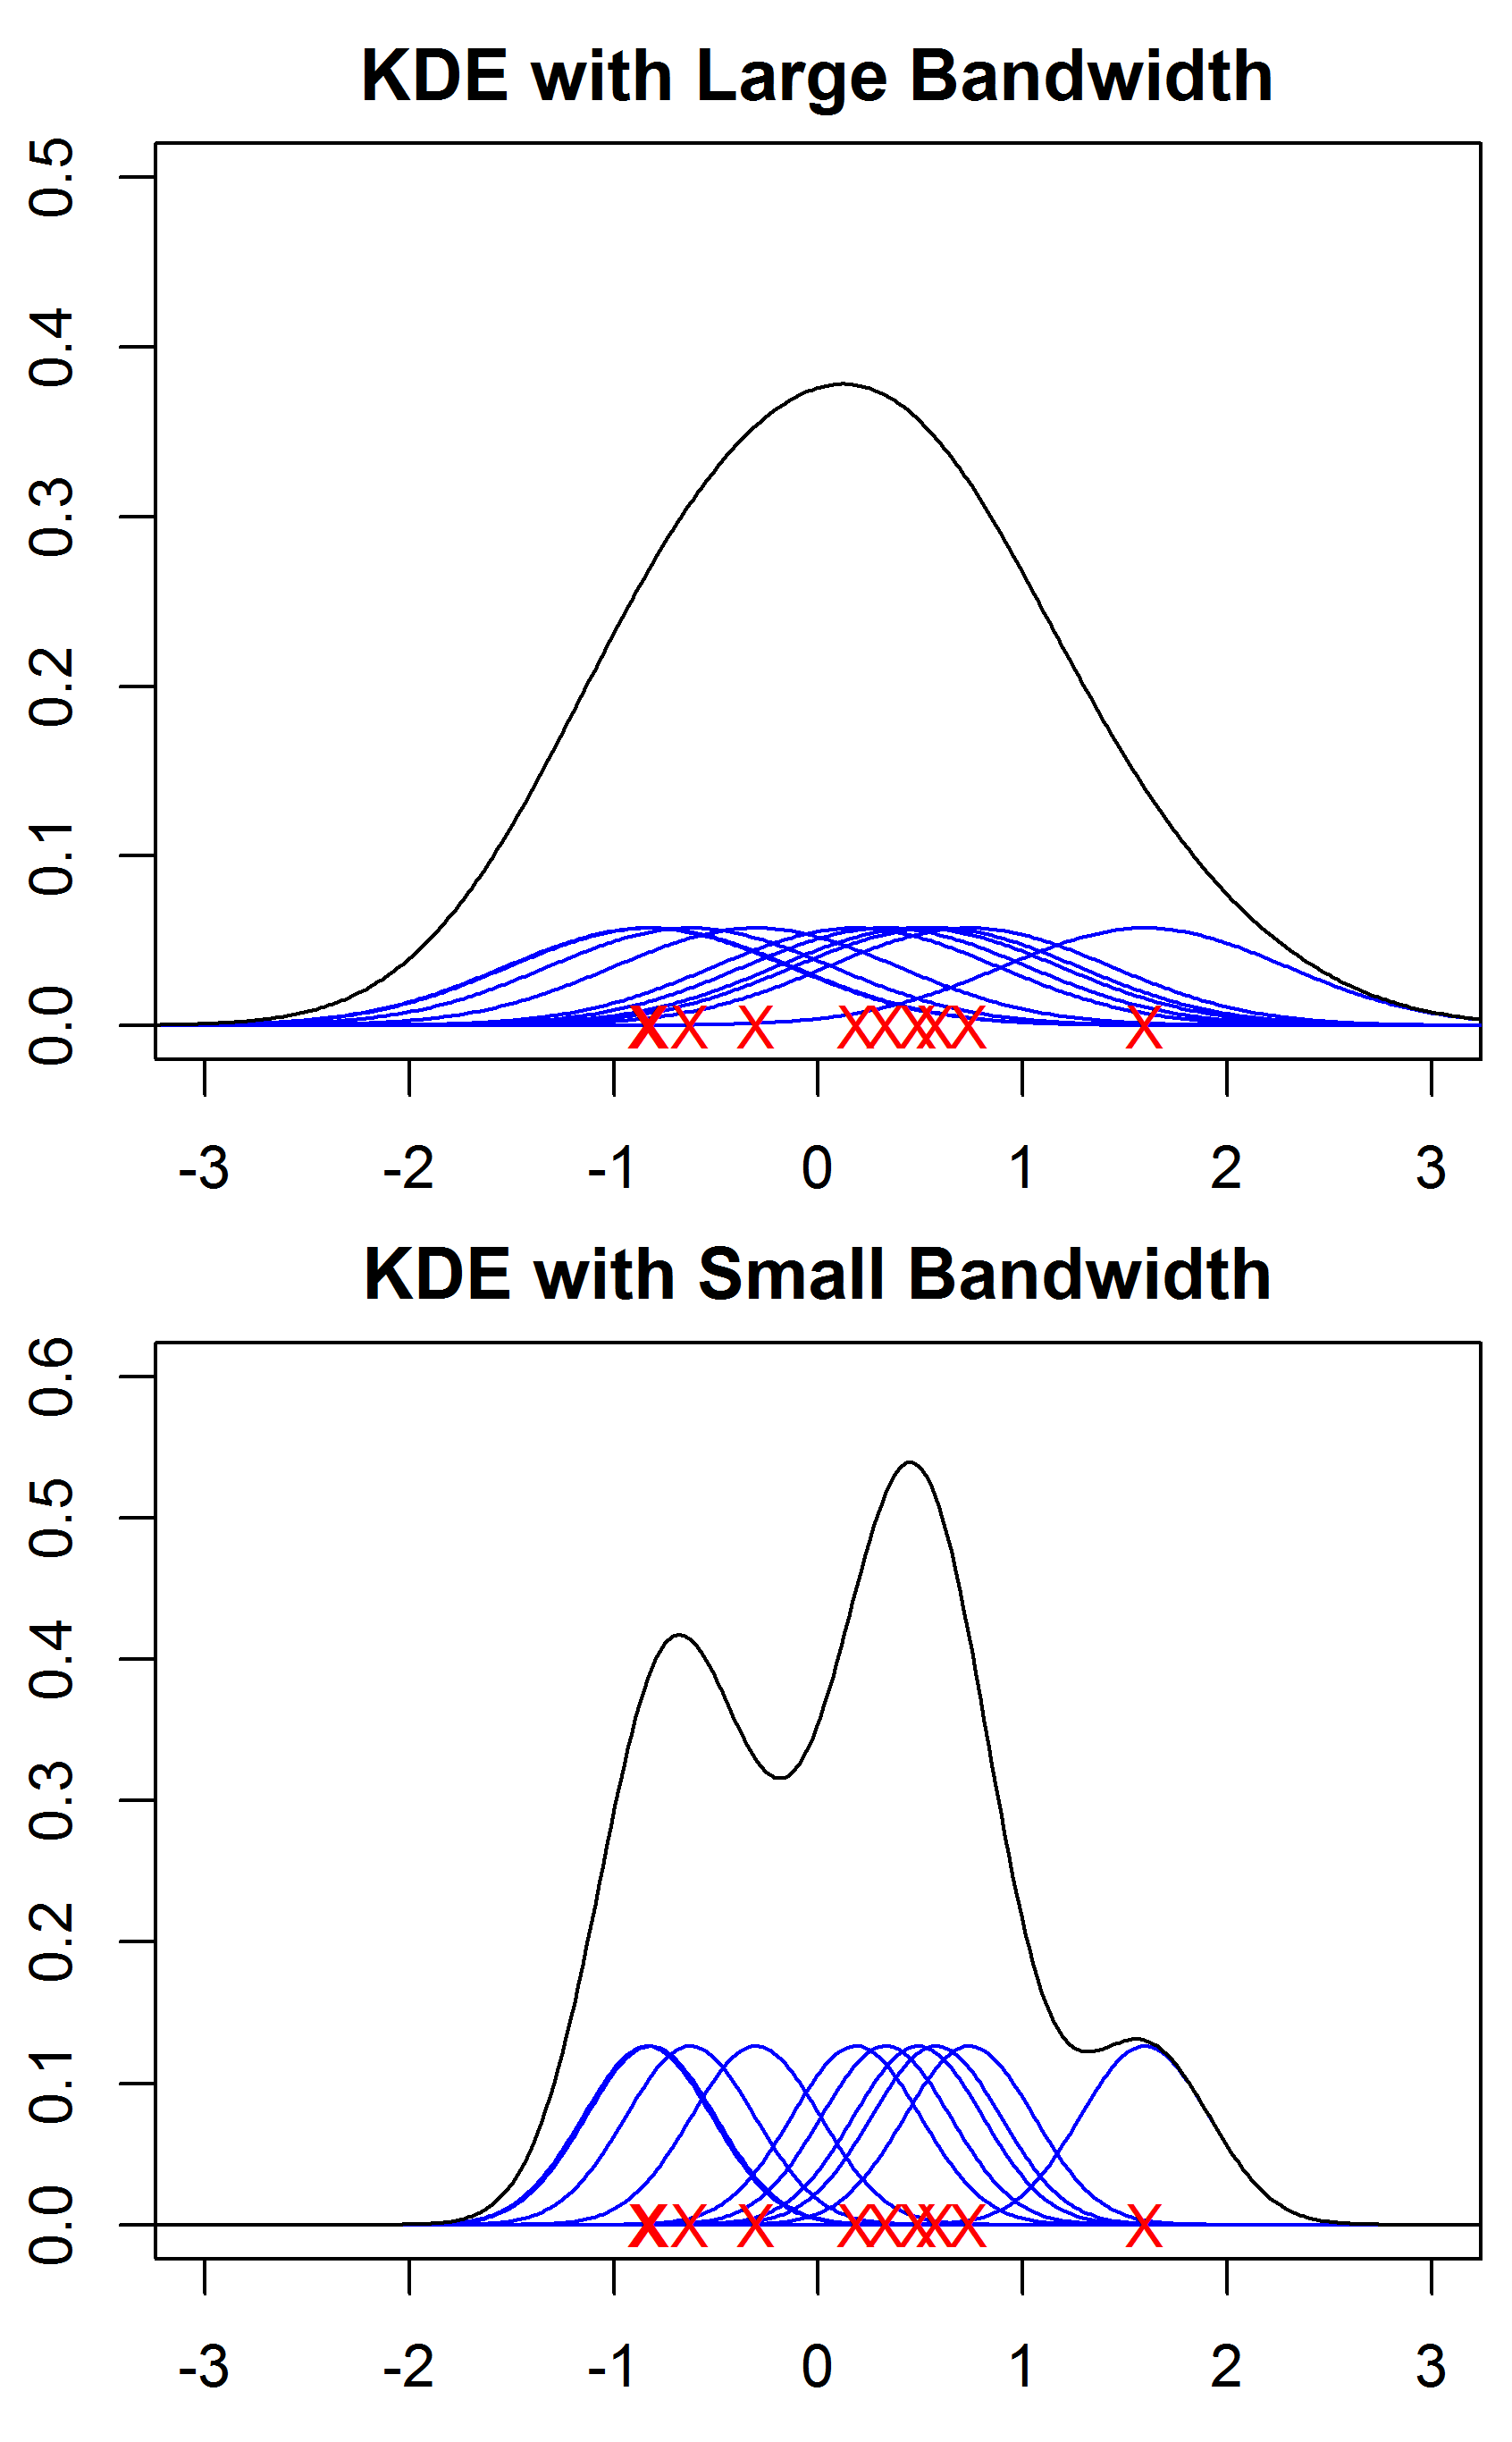
\includegraphics[width = 7in]{KDEDemo.png}
     \centering
     \end{figure}
\end{column}
\end{columns}

\end{frame}

\begin{frame}{Candidate Bandwidths (1/2)}

\begin{block}{Unbiased Cross Validation (E{[}UCV + R(f){]} = MISE)}

Minimize

\[
UCV(h) = R\left(\widehat{f}\right) - \frac{2}{n} \sum_{i = 1}^{n} \widehat{f}_{-i}(x_i)
\] instead.

\[
\widehat{f}_{-i}(x_i) = \frac{1}{h(n-1)}\sum_{j \neq i} K\left(\frac{x_i - x_j}{h}\right)
\]

is the LOO estimator. Used to estimate the second term in
\(ISE(h) = \int \widehat{f}^2 - 2 \int\widehat{f}_h f + \int f^2\).

Issue: excessive variation

\end{block}

\end{frame}

\begin{frame}{Candidate Bandwidths (2/2)}

\begin{block}{Terrell's Maximal Smoothing}

Instead of estimating \(R(f^{''})\), what if we tried to minimize it?
Built on the result that the \(beta(k + 2, k + 2)\) family minimizes
\(\int (f^{(k)})^2\) for a given standard deviation.

\[
h_{MS} =  3 \hat \sigma \left(\frac{R(K)}{35 n} \right)^{\frac{1}{5}}
\] Issue: upper bound on \(h_{opt}\) \(\rightarrow\) oversmooths
interesting features of the data

\end{block}

\end{frame}

\begin{frame}{Example 1}

50/50 mixture of \(N(0,1)\) and \(N(2, 2^2)\)

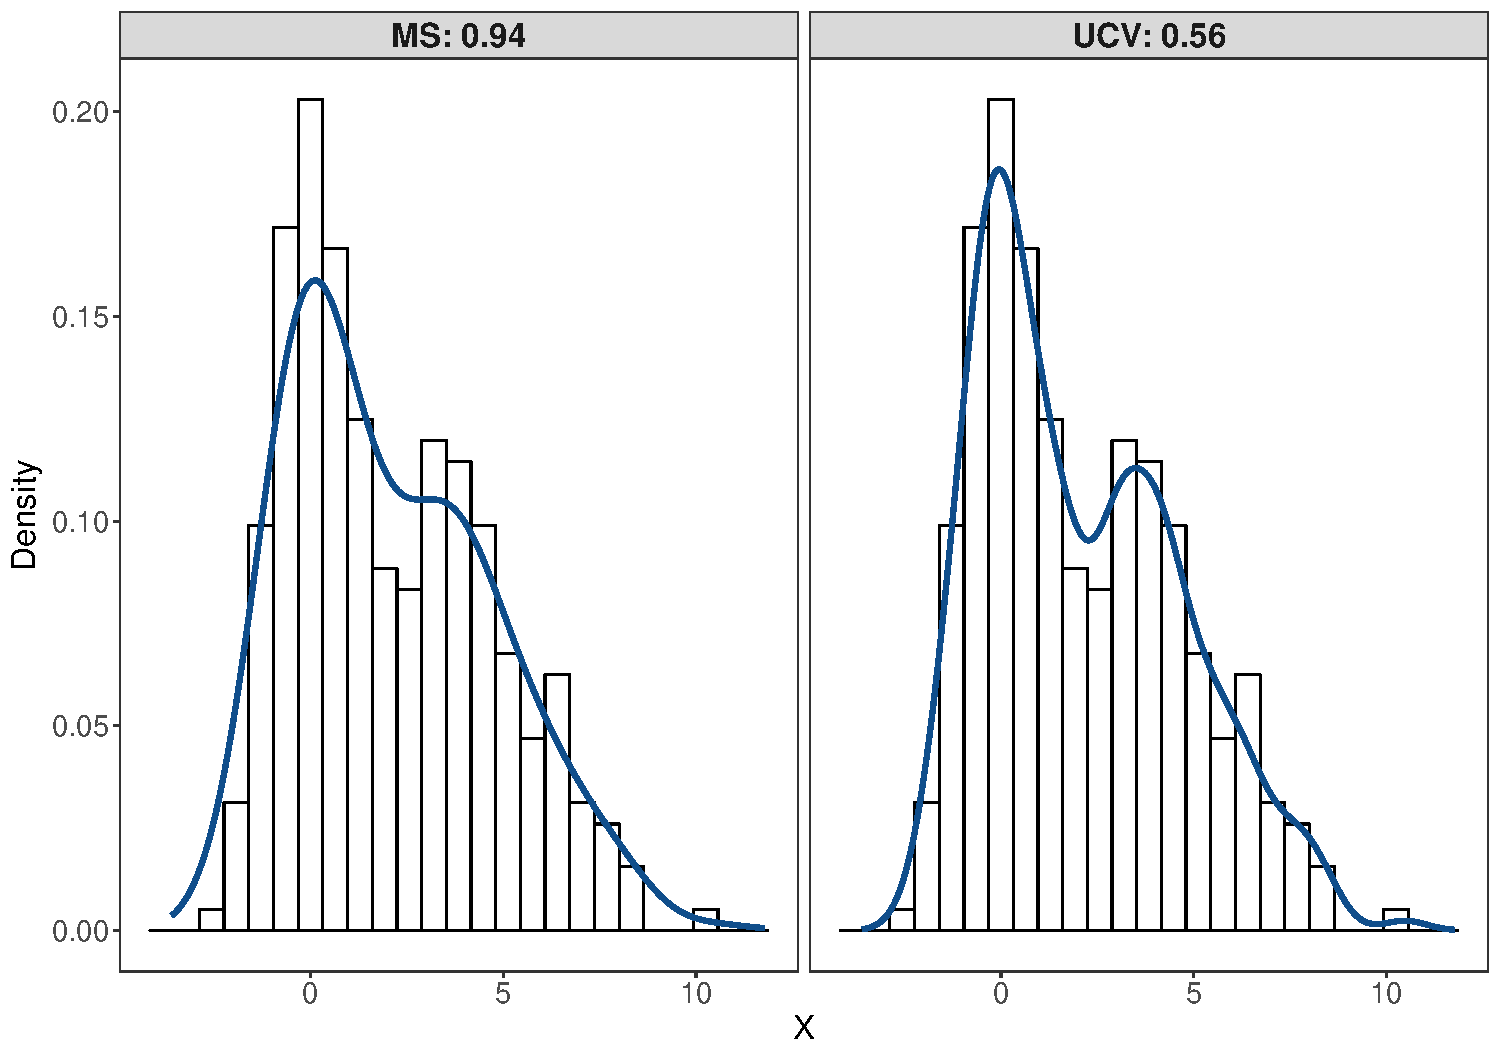
\includegraphics{ProjectPresentation_files/figure-beamer/unnamed-chunk-2-1.pdf}

--\textgreater{}

\end{frame}

\begin{frame}{Example 2}

Alcohol by volume of Beer Advocate's top 250 beers

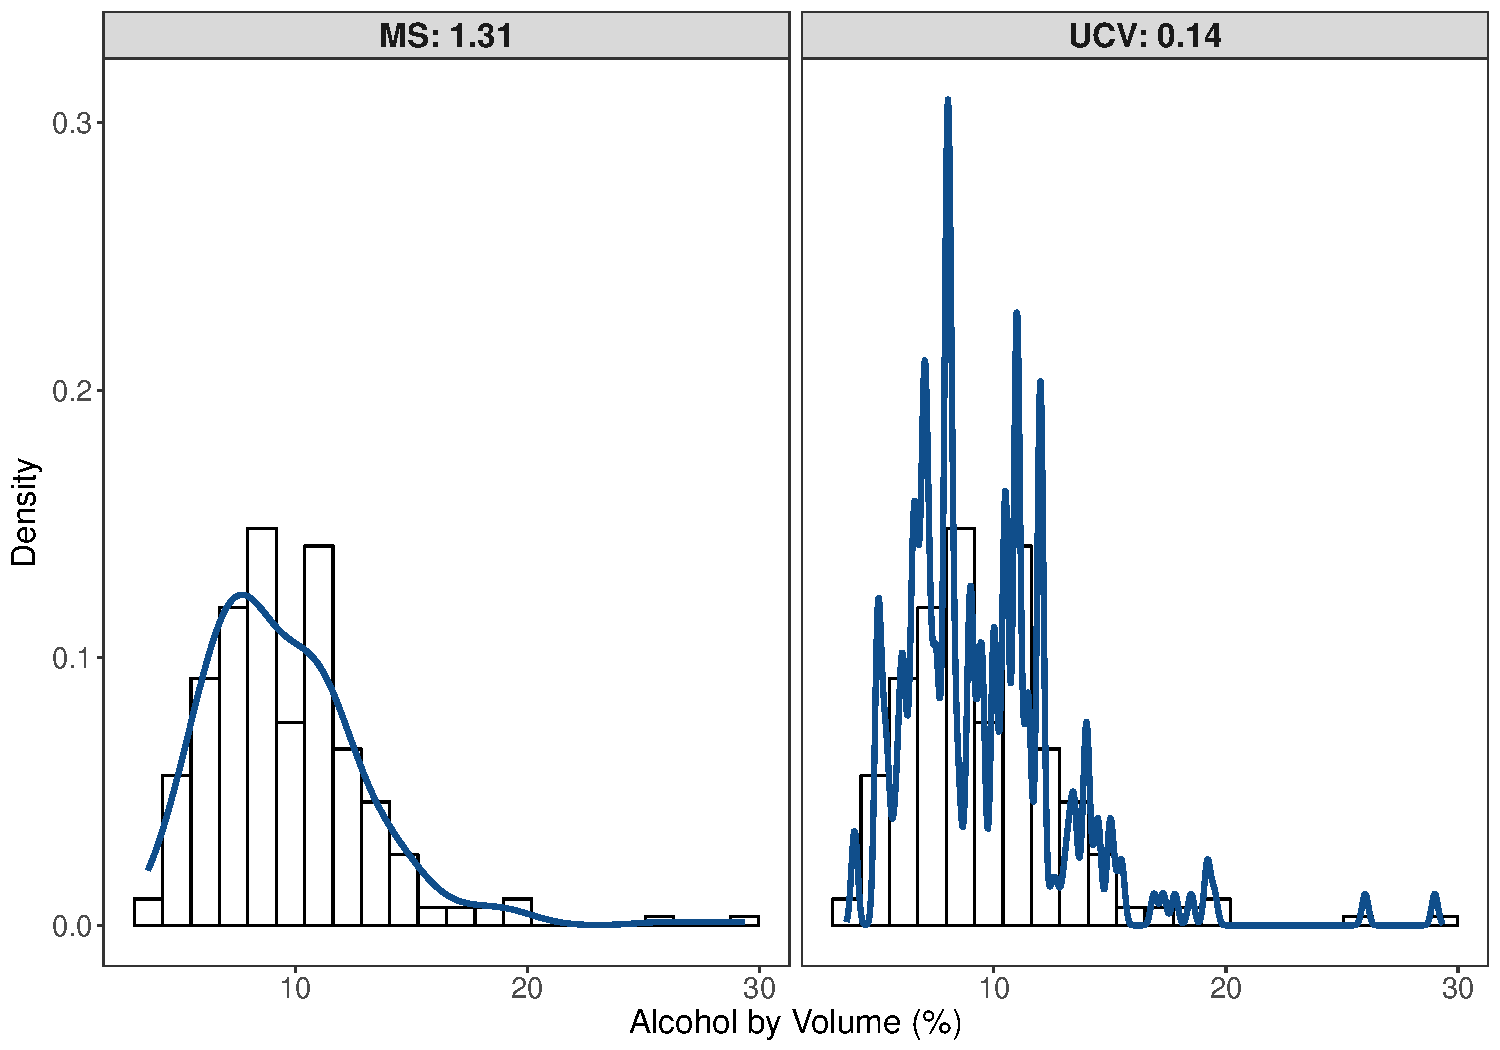
\includegraphics{ProjectPresentation_files/figure-beamer/unnamed-chunk-4-1.pdf}

\end{frame}

\begin{frame}{Conclusion}

\begin{itemize}
\tightlist
\item
  Choosing a bandwidth should be an iterative process
\item
  Bias - variance tradeoff

  \begin{itemize}
  \tightlist
  \item
    Too smooth: low variance, high bias

    \begin{itemize}
    \tightlist
    \item
      what \emph{is not there} might be
    \end{itemize}
  \item
    Too wiggly: high variance, low bias

    \begin{itemize}
    \tightlist
    \item
      what \emph{is there} might be too hard to see
    \end{itemize}
  \end{itemize}
\end{itemize}

\end{frame}

\end{document}
